\chapter{Soluzione Proposta}

\begin{citazione}
    In questo capitolo vengono discusse le motivazioni dietro la scelta del protocollo \emph{CAN}, nonchè delle problematiche riscontrate nel protocollo e di come può essere possibile risolverle
\end{citazione}

\section{Scelta del protocollo}
Al fine di procedere con il lavoro di messa in sicurezza è stato necessario scegliere uno dei protocolli \emph{Automotive} disponibili in letteratura. La prima scelta è stata \emph{FlexRay} in quanto è il protocollo più promettente e con hardware più prestante ma, sfortunatamente, dopo un'attenta ricerca in rete non è stata trovata nessuna implementazione software del protocollo. Erano disponibili solo all'acquisto delle \emph{board di testing} (con costi anche abbastanza sostanziosi) che permettevano di simulare il protocollo tramite strumentazione adeguata. Non avendo avuto fortuna con \emph{FlexRay}, la seconda scelta è ricaduta su \emph{LIN}. Purtroppo anche qui non è stato possibili trovare implementazioni \textbf{funzionanti} e \textbf{complete} del protocollo, ma solo tentativi abbandonati di implementarlo. Per queste ragioni, infine, si è scelto il protocollo \textbf{\emph{CAN}} che è supportato in maniera nativa dal kernel \textbf{Linux} tramite dei moduli appositi (oltre ad avere anche diverse implementazioni software complete e funzionanti), permettendo persino la creazione di uno o più nodi virtuali.

\section{Problematiche di sicurezza riscontrate}
Nonostante \emph{CAN} sia uno dei protocolli più utilizzati nell'ambito \emph{Automotive}, questo presenta gravi vulnerabilità di sicurezza. Soprattutto, i problemi principali sono due:
\begin{itemize}
    \item Assenza di qualunque meccanismo di \textbf{protezione del payload} dei messaggi, lasciandolo vulnerabile a modifiche maliziose e all'intercettazione;
    \item Assenza di un qualunque meccanismo di \textbf{autenticazione} dei nodi, permettendo a chiunque si connetta alla rete di inviare e leggere dati, permettendo anche l'invio di \textbf{messaggi falsi} e l'invio di un grande numero di messaggi \emph{spazzatura} con lo scopo di disturbare la rete o renderla \textbf{non disponibile}.
\end{itemize}

Questa situazione è originata dal fatto che i creatori del protocollo hanno posto l'attenzione soprattutto sulle \textbf{prestazioni}, tralasciando gli aspetti di sicurezza. Il motivo dietro questa scelta è che, essendo utilizzato in un ambiente \emph{safety-critical}, introducendo dei ritardi nella comunicazione si generano dei rischi all'incolumità delle persone all'interno delle auto in cui è utilizzato \emph{CAN}, nonchè di quelle nelle vicinanze, sfociando così in una situazione \textbf{inaccettabile}. Se si pensa ad un sistema \textbf{Steer-by-wire}, nel quale una \emph{ECU} controlla la rotazione delle ruote in base al movimento dello sterzo, un ritardo tra movimento dello sterzo e rotazione \emph{effettiva} delle ruote potrebbe tramutarsi in un impatto con un oggetto (edificio, veicolo, ecc.) o persona.

\section{Soluzione proposta}
Per cercare di risolvere il problema della mancanza di \textbf{protezione del payload} all'interno del protocollo \emph{CAN}, quello che si è voluto proporre è l'\textbf{aggiunta di uno strato di cifratura} che protegga lo scambio di messaggi sulla rete. Una soluzione abbastanza banale può essere quella di decidere, in fase di configurazione della rete, una chiave di cifratura e utilizzare \textbf{sempre} quella per inviare messaggi cifrati, tuttavia, una soluzione del genere è inaccettabile per molti motivi, tra cui:
\begin{itemize}
    \item Per poter utilizzare questa chiave è necessario che essa venga salvata, per cui è necessario utilizzare hardware apposito in maniera tale da salvarla \textbf{in modo sicuro};
    \item Considerando che la vita media di un veicolo può superare i 10 anni, usare la stessa chiave così a lungo diventa problematico, in quanto, durante un periodo di tempo così lungo la rottura della chiave può essere plausibile e questo rende completamente vano l'utilizzo della cifratura, anche per messaggi già inviati in precedenza;
\end{itemize}

Quindi è necessario trovare un modo che permetta di \textbf{non dover salvare la chiave} e che consenta un \textbf{aggiornamento della chiave da utilizzare}, in modo tale da evitare modifiche alle \emph{ECU} (rendendo la soluzione \textbf{retrocompatibile} con le automobili già in commercio) e far si che in caso di violazione della chiave sia compromessa solo una sessione e non tutte.\\
Il modo migliore per garantire queste due caratteristiche è l'utilizzo di un \textbf{cifrario ibrido}, ovvero un cifrario che ha una componente asimmetrica per far accordare i nodi su una stessa chiave di sessione e che ha una componente simmetrica con la quale viene utilizzata la chiave di sessione come chiave di cifratura per i messaggi che devono essere scambiati. Uno schema riassuntivo di ciò che vuole introdurre la soluzione si può consultare nella \autoref{fig:can-protection}.

\begin{figure}[h]
    \begin{subfigure}{0.45\textwidth}
        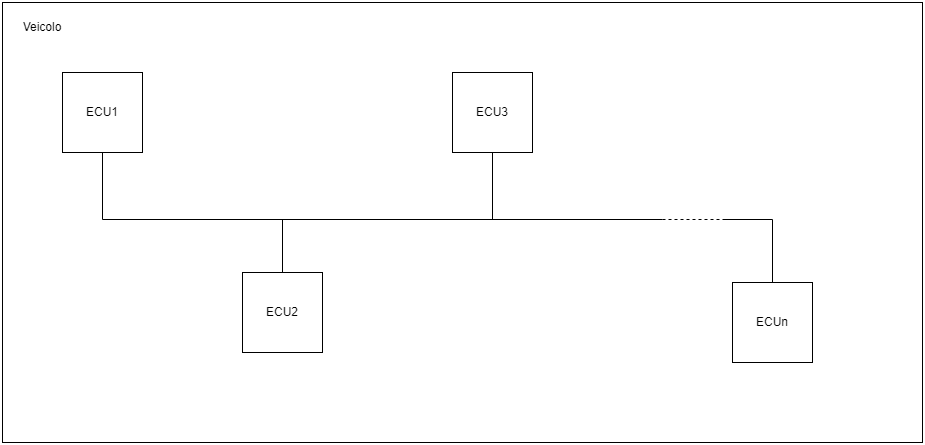
\includegraphics[width=1\textwidth]{capitoli/figure-soluzione-proposta/can-no-protection.png}
        \vspace{0.7cm}
        \caption{\emph{CAN} senza nessuna protezione}
        \label{fig:can-no-protection}
    \end{subfigure}
    \hfill
    \begin{subfigure}{0.45\textwidth}
        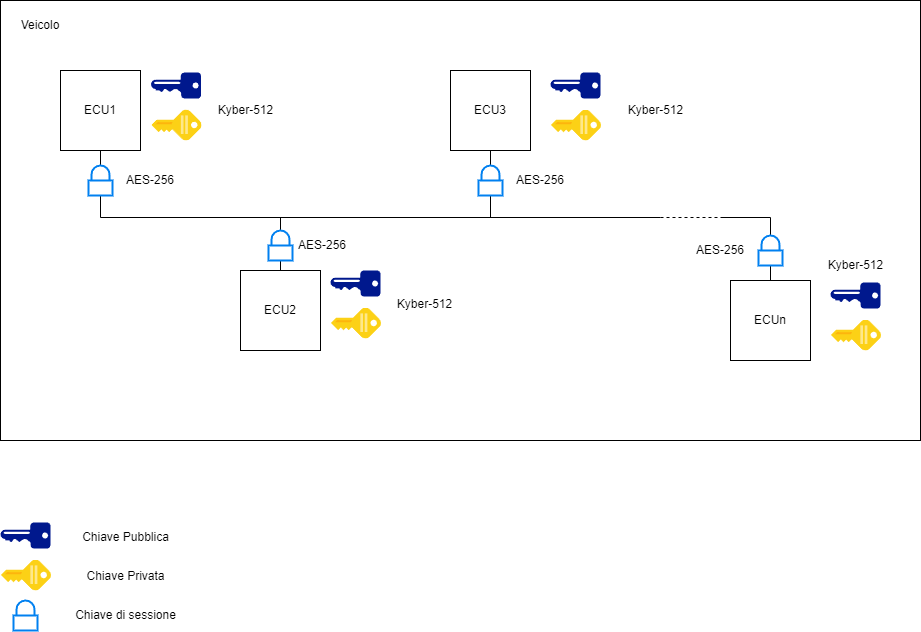
\includegraphics[width=1\textwidth]{capitoli/figure-soluzione-proposta/can-with-protection.png}
        \caption{\emph{CAN} con l'utilizzo di un \textbf{cifrario ibrido}}
        \label{fig:can-with-protection}
    \end{subfigure}
    \caption{Schema di \emph{CAN} senza e con l'aggiunta di un \textbf{cifrario ibrido}}
    \label{fig:can-protection}
\end{figure}

\subsection{Scelta degli algoritmi di cifratura}
Per poter realizzare il \textbf{cifrario ibrido} citato in precedenza, è necessario scegliere due algoritmi di cifratura: uno \emph{simmetrico} e uno \emph{asimmetrico}. In particolare, si è deciso di impiegare cifrari appartenenti alla categoria \textbf{Post-Quantum} con il fine di garantire la massima sicurezza contro la maggior parte degli attacchi noti in letteratura e garantire anche la sicurezza contro un attacco da parte di un computer quantistico.\\
In seguito a questa decisione, quindi, si è deciso di impiegare come algorimto \emph{simmetrico} il cifrario \textbf{AES-256} mentre come algoritmo \emph{asimmetrico} il \emph{KEM} \textbf{CRYSTALS-kyber-512}.

\subsection{Funzionamento della soluzione}
Una delle caratteristiche che si vogliono garantire con l'introduzione del \textbf{cifrario ibrido}, come citato in precedenza, è la \textbf{retrocompatibilità} con le \emph{ECU} che non adottano la soluzione, in modo tale da estendere la soluzione proposta a quante più auto possibile.\\
Il modo migliore per garantire questa caratteristica è quella di \textbf{non modificare il protocollo}, senza alterarne nè la struttura nè i messaggi scambiati e senza applicare modifiche all'hardware necessario. Quindi, l'aggiunta del cifrario non può avvenire a livello di protocollo (implicherebbe una modifica a \emph{CAN}) ma deve avvenire a livello di \textbf{applicazione}. L'idea è quella di far sì che l'applicativo sull'\emph{ECU} effettui la cifratura del payload \textbf{prima} che questo venga inviato come messaggio tramite \emph{CAN}. In questo modo, il payload che viaggia \emph{in chiaro} è in realtà un payload cifrato che verrà decifrato dalla \emph{ECU} interessata, senza il rischio che un attaccante possa fare \textbf{eavesdropping} del messaggio.

Per poter realizzare un sistema del genere, è necessario creare un \textbf{protocollo} che si occupi di:
\begin{itemize}
    \item Generare una coppia di chiavi;
    \item Scambiare una chiave di sessione;
    \item Cifrare un messaggio;
    \item Decifrare un messaggio.
\end{itemize}

Tutto questo, ovviamente, senza aggiungere nuove tipologie di messaggi e senza alterare gli ID \emph{CAN} disponibili, in modo da non causare incompatibilità con \emph{CAN}. Quindi, un possibile protocollo che riesca ad occuparsi di tutti i compiti citati può essere la seguente sequenza di passi:
\begin{enumerate}
    \item Generazione di una coppia di chiavi \emph{asimmetriche};
    \item Scambio della chiave pubblica;
    \item Generazione di una chiave di sessione;
    \item Scambio e salvataggio della chiave di sessione;
    \item Cifratura e decifratura del traffico.
\end{enumerate}

Un sequence diagram che chiarisce il funzionamento può essere visto in \autoref{fig:sequence-diagram-protocol}.
\begin{figure}[h]
    \centering
    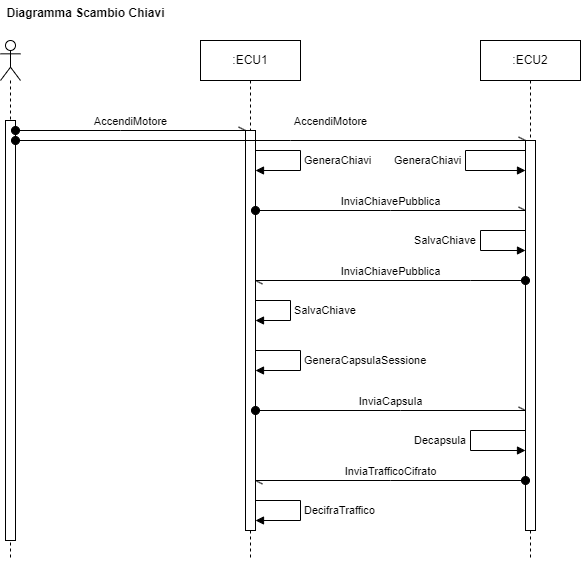
\includegraphics[width=0.8\textwidth]{capitoli/figure-soluzione-proposta/sequence-key-exchange.png}
    \caption{Sequence Diagram del protocollo proposto}
    \label{fig:sequence-diagram-protocol}
\end{figure}

Riuscendo ad implementare il protocollo proposto senza dover necessariamente alterare caratteristiche di \emph{CAN}, permetterebbe di riuscire a \textbf{proteggere il payload} e raggiungere l'obiettivo fissato per il lavoro.